\documentclass[a4paper,12pt]{article}
\usepackage[T2A]{fontenc}
\usepackage[utf8x]{inputenc}
\usepackage[english,russian]{babel}
\usepackage{amsmath,amssymb,amsfonts}

\usepackage[labelfont=bf,labelsep=period]{caption}
\usepackage{subfig}
\usepackage{pgfmath}
\usepackage{tikz}
\usetikzlibrary{arrows,fit,positioning,shapes.multipart}
\usepackage{fullpage}

\begin{document}
	\thispagestyle{empty}

\renewcommand{\thesubfigure}{\asbuk{subfigure}}

\begin{figure}
	\subfloat[течение Куэтта]{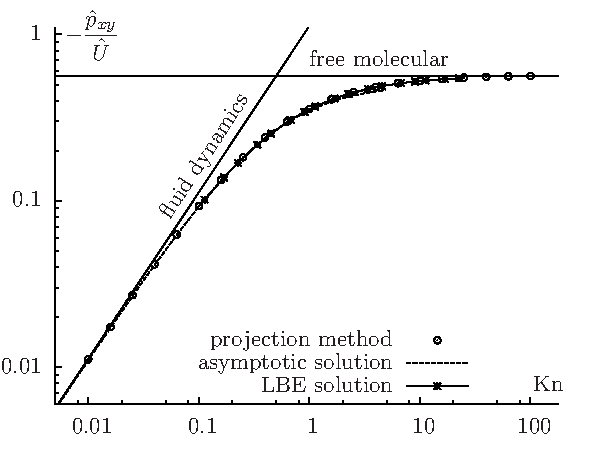
\includegraphics[width=0.5\textwidth]{couette}}
	\subfloat[перенос тепла]{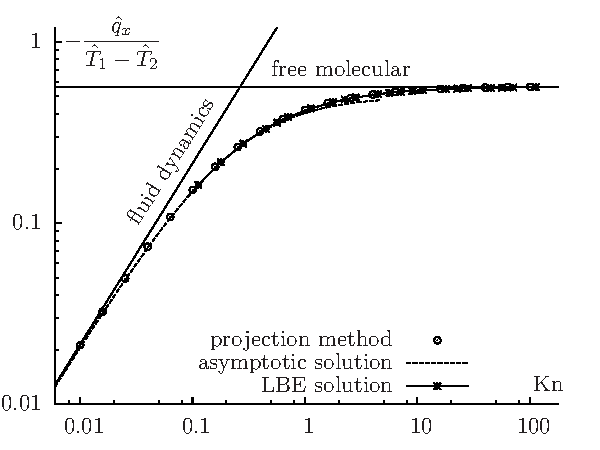
\includegraphics[width=0.5\textwidth]{heat}}
\end{figure}

\end{document}
